\documentclass[conference]{IEEEtran}
\hyphenation{op-tical net-works semi-conduc-tor}
\usepackage{hyperref}
\usepackage{graphicx}
\usepackage{float}
\usepackage{caption}
\usepackage{subcaption}
\usepackage{tikz}
\usepackage{fixltx2e}
\usepackage{listings}
\restylefloat{table}
\floatstyle{boxed}
\restylefloat{figure}
\definecolor{mygray}{rgb}{0.7,1.2,0.7}
\graphicspath{ {images/} }
\DeclareGraphicsExtensions{.pdf,.png,.jpg}
\lstset{captionpos=b,backgroundcolor=\color{mygray},caption={Snippet of labspec.json file}}
\begin{document}

\title{Any Time Virtual Labs: \\ On Portable Media and As Debian Packages}


\author{\IEEEauthorblockN{Nurendra Choudhary}
\IEEEauthorblockA{International Institute of Information Technology,\\
Hyderabad, India\\
Email: nurendrachoudhary31@gmail.com}
\and
\IEEEauthorblockN{Dr. Venkatesh Chopella}
\IEEEauthorblockA{International Institute of Information Technology,\\
Hyderabad, India\\
Email: venkatesh.choppella@iiit.ac.in}
}

\maketitle


\begin{abstract}
\textbf{As education and technology merge, the diversity of teaching and learning methods expand even more.\\
  This paper proposes a novel method to bring the engineering students closer to their specific fields of interest. Many engineering students lack access to decent labs. Our aim is to provide such students with Virtual Labs which are easily accessible and work without network connectivity.\\
  Virtual Labs are web applications which use various programs to provide in-lab experience to their users. The proposal is to preinstall the virtual labs with full environment on an Operating System. Also, Debian packages will be provided for easy installation of the labs on existing Operating System.
}     
\end{abstract}

\IEEEpeerreviewmaketitle


  \section{Introduction}
  Laboratories play a pivotal role in engineering studies. The laboratory experience of using instruments and materials encourages students in exploring and building advanced skills through self motivated discovery learning \cite{desico}. However, many of experiments cant be conducted in real life laboratory setting for variety of reasons like cost, unavailability of resources and the risks involved. Unfortunately, many colleges and schools across the world lack the presence of labs at their disposal. As a result, governments and educational organizations are now taking initiatives in setting up virtual laboratories to augment current learning infrastructure.
  \\
  Virtual labs represent a way to convey and learn subjects using the power of visualizations and computer generated simulations. Physical science experiments can now easily be simulated in a virtual environment without any fear of a physical damage and at a relatively low cost. A virtual lab also includes a highly supportive learning environment to help interested students in exploring the experiment topic in more depth. Every virtual lab contains learning material describing the objective, theory behind the experiment, an instruction manual to guide students in the experiment, quizzes and most importantly an environment for conducting experiments \cite{discovir}.
  \\
  Physically, a Virtual Lab is a directory containing the web application for running the lab and various other support files which contain the specifications of the lab for future support for the developers.\\
  However, this idea also had certain limitations. It required network connectivity which is very limited and sometimes non-existent in the developing and under-developed parts of the world. Also, setting up the client side environment in the machine was no easy task. It required a good knowledge of support applications. This limited the access to those with a good background in computers.\\
  To handle these limitations, we tried to integrate the network requirements of the Virtual Labs to the local system itself. We created Operating Systems with all the server-side and client-side technical dependencies preinstalled in them. Then, we setup all the Virtual Labs in the Operating Systems. After that, we configured the Operating System to be able to host all the virtual labs on its local server without any necessity for external support. For making the Debian packages, individual labs were taken and their Debian packaging files were modified a way that all the dependencies and support files were included properly. This confirmed the working of the labs on the system with no further modifications required to be made by the user.\\
  This solution has been currently tested and implemented with 17 virtual labs of diverse fields of different  universities with successful results.\\
    \begin{figure*}
    \begin{subfigure}{2\columnwidth}
      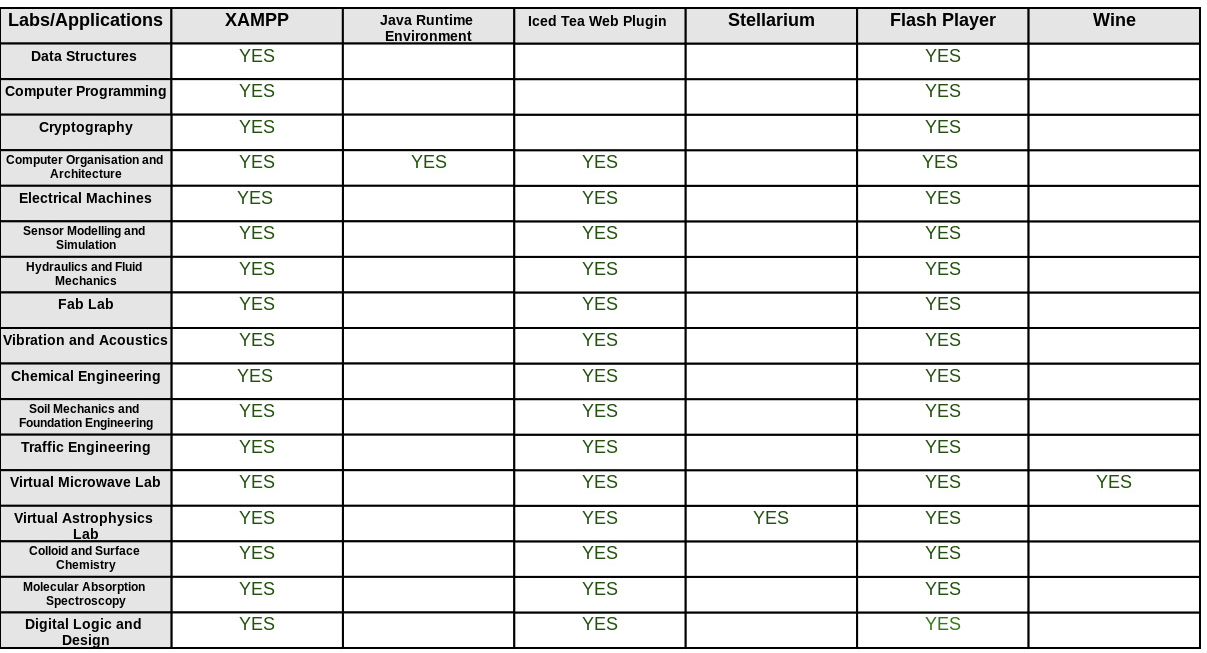
\includegraphics[width=1.04\textwidth,height=0.7\textwidth]{table.png}
    \end{subfigure}
    \caption{Application requirements of various labs}
    \label{fig:appreq}
\end{figure*}
\section{Approach}
   Note: labspec.json is a file inside every lab which specifies the requirements of the given lab. All dependencies of the labs are referred from this file.
  \begin{lstlisting}[frame=single]
........Rest of the code........  
  "type": ""
}, 
"runtime_requirements": {
  "platform": {
  "arch": "i386", 
  "hosting": "dedicated", 
  "installer": ["sudo apt-get update"
              ,"sudo apt-get install 
                -y php5 apache2"
               ], 
  "lab_actions": {
  "init": ["mv /var/www/index.html 
            index.html.default",
            "cp -r ../build/* 
            /var/www/"
          ], 
  "pause": [], 
  "resume": [], 
  "shutdown":["service apache2 stop"], 
  "start":["service apache2 start"],  
  }, 
  "memory": {
........Rest of the Code........
  \end{lstlisting}
  As we can observe the file contains \textbf{JSON} objects. Inside the object \textit{"runtime requirements"} in the object \textit{"installer"}, we have the set of commands which are required to install the server-side requirements of the Virtual Lab. This was used to get the server-side requirements of the Lab.
  \subsection{Building the Customised Operating System:}
  \begin{figure*}
    \begin{subfigure}{\columnwidth}
      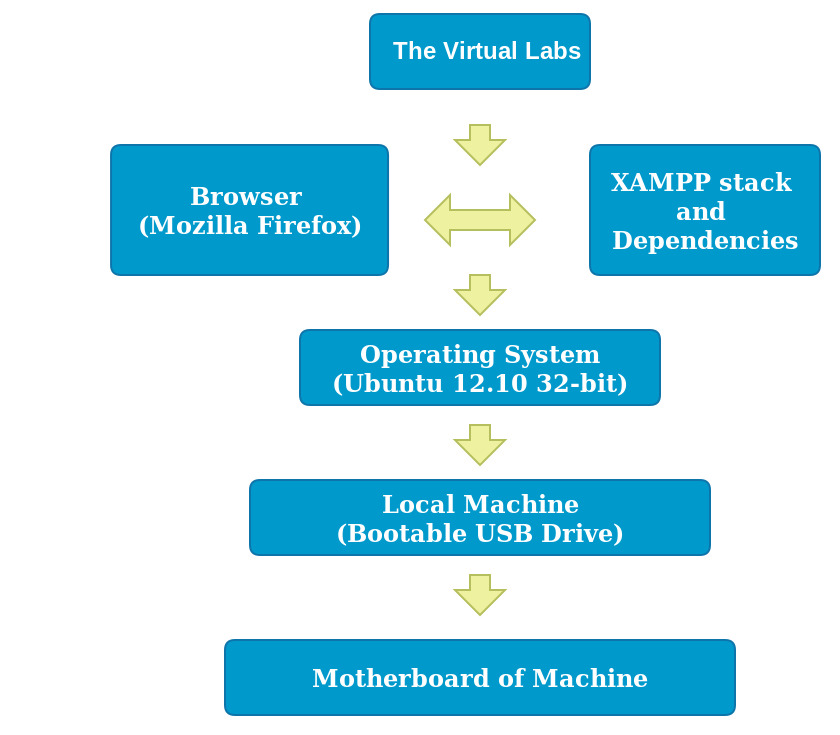
\includegraphics[width=0.8\textwidth,height=1.35\textwidth]{portable_usb}
      \caption{Abstraction Layer of the Customised Ubuntu}
    \end{subfigure} 
    ~
    \begin{subfigure}{\columnwidth}
     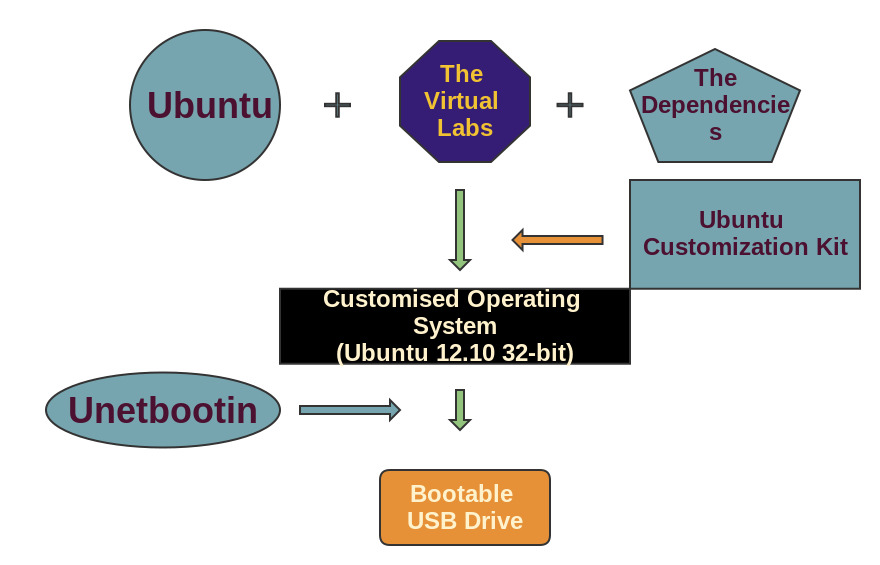
\includegraphics[width=0.8\textwidth,height=1.35\textwidth]{project1}
     \caption{Making the Customised Ubuntu}
    \end{subfigure}
    \caption{Making the Portable Media with preinstalled Virtual Labs.}
\end{figure*}
  Operating System is the basic way of communication between the man and the machine for any average computer user. So, the first part of the project aims at developing an Operating System with all the Virtual Labs and a fully functional support environment for the labs preinstalled. This will primarily remove the necessity of a network in using the labs and also help reduce a significant amount of labour carried out in installing the environment.\\    
  Firstly, we needed a base Operating System which is easily customisable and available universally. For this, Ubuntu was decided upon as the best option.\\ One of the major aims of the project is to make the technology accessible to the maximum number of students. Ubuntu, apart from being one of the widely used Operating Systems in engineering, is also a freeware. This significantly increases the outreach of this new technology to the classes with weak financial conditions.\\
  After this, we needed we needed an application that is able to customise the root of a base Ubuntu image and be able to install the extra packages needed in the image itself. For this, we chose an application called \textbf{Ubuntu Customisation Kit} that is available in the \textit{Ubuntu Software Centre} as a freeware.\\ 
  Our first target for this project was to integrate the server and the machine. So, we set out by using basic applications for implementing local servers and databases, i.e, \textbf{php5}, \textbf{apache2} and \textbf{MySQL}. We realised later in the project that these applications are not able to support many labs. So we switched to XAMPP stack for handling the local server and databases on the system. With this, we were able to meet the server-side requirements of the labs.\\
  The next major task was to setup the Virtual Labs on the Ubuntu image. To accomplish this, we took all the labs (which are directories as mentioned earlier in the Introduction section) and put them in the directory created by XAMPP for hosting the web application(\textit{/opt/lampp/htdocs/}). This step confirmed that the web applications will be properly hosted on the localhost.\\
  The final step was to setup the client-side environment on the system to run all the labs with full functionality. This is the most difficult step of the entire process as different labs require different applications for their support. Also the lab specifications of the lab only mentioned the server-side requirements. So, we had to start out by checking each and every page and experiment of the labs to find out its client-side dependencies. The results we found out are as follows.
    In figure~\ref{fig:appreq}, we can clearly observe the diversity of applications that are needed for the client-side of the Virtual Labs. This is clearly a task that is very difficult for a normal first-time user. We have now recognized the dependencies, so we started installing them on the system. This is the step where we found out that the application \textit{Wine} is not compatible with php5 and apache2 combination and so we switched to XAMPP stack.\\
    A lot of problems occurred during the switch to XAMPP stack. Firstly, automatic installation of XAMPP stack was not available for Ubuntu-12.10. So we did a manual installation using \textit{tar} files and then configured it manually for the Ubuntu-12.10 system for which we had to study XAMPP from the scratch. This resulted in the proper running of the \textit{Wine} application.\\
    But then due to XAMPP, the previously installed default flashplayer plugin stopped working. So, we had to search for its alternatives too and install and setup the plugin manually. The next challenge was running the .jnlp files which were not supported by the Ubuntu default browser, i.e, Mozilla Firefox. To take care of this problem we had to setup Java Environment on the system and also load the \textit{Icedtea web plugin} for supporting the java .jnlp files on the browser. Then we tried running again. But it had supported issues with a 64-bit architecture. So we had to switch to a 32-bit system and repeat the whole process. This time it worked properly. Next, we installed the Stellarium package which a comparatively easier task. \\\
    After all these major steps, our Virtual Labs were fully functional on the system. But then, this project was designed for making the users comfortable. So, some small changes were made for better user experience. These changes included starting the local XAMPP server upon boot and setting the default page of Firefox(the default browser) to \textbf{http://localhost/} which hosted the Virtual Labs. Refer \cite {MFH}\\
   Finally, all these changes were appropriately made using \textbf{Ubuntu Customization Kit} and the Customised Ubuntu Operating System was ready.\\
   \textbf{ Note: The above procedure is just an outline. For more details, refer the full documentation \cite {COSI}}\\
   \textbf{For the latest version of this Customised Operating System, refer \cite {COS}.}\\ 
  \subsection{Building the Debian Packages:}
  %\end{multicols}
  \begin{figure*}
    \begin{subfigure}{\columnwidth}
      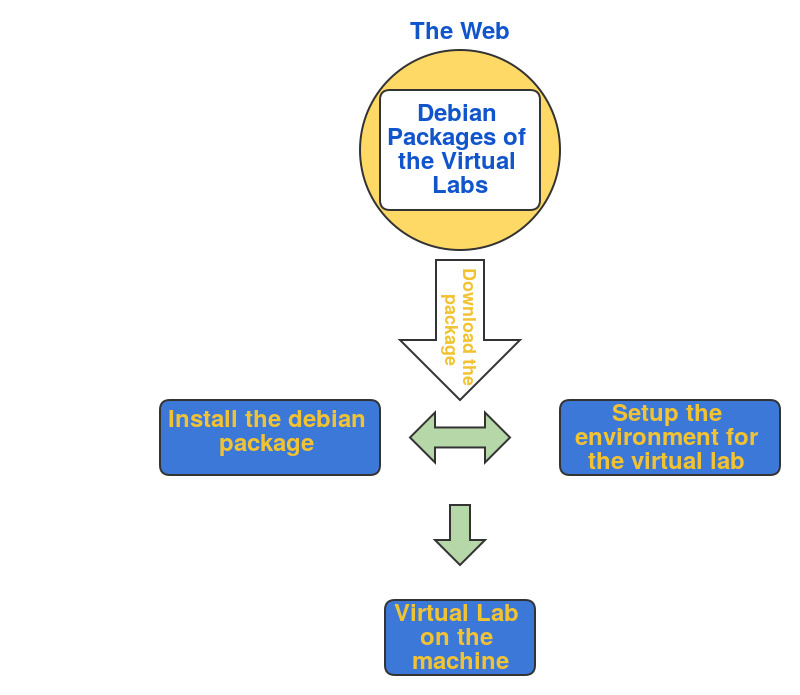
\includegraphics[width=0.9\textwidth,height=1.4\textwidth]{debian_packaging}
      \caption{Making Debian Packages}
    \end{subfigure} 
    ~
    \begin{subfigure}{\columnwidth}
      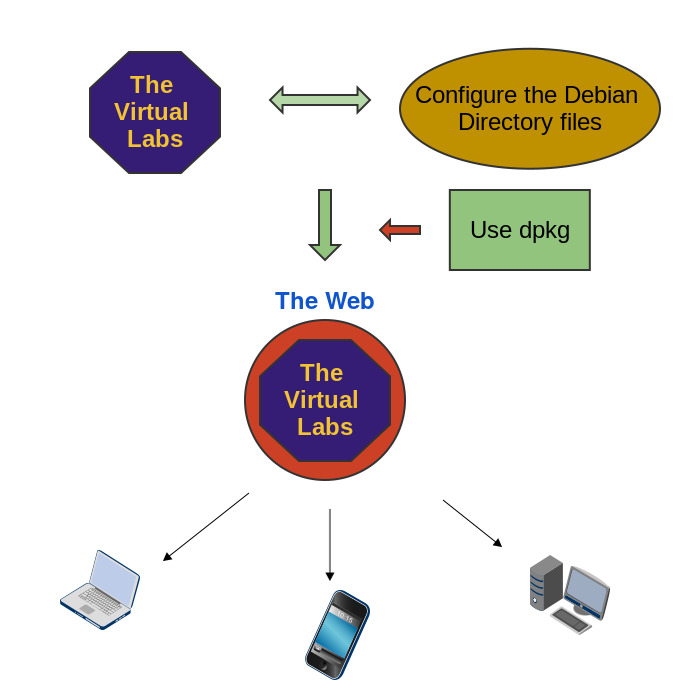
\includegraphics[width=0.9\textwidth,height=1.4\textwidth]{debpack}
      \caption{Debian Packages in use}
    \end{subfigure}
    \caption{Debian Packaging of the Labs}
\end{figure*}
%\begin{multicols}{2}
  Debian Packages are built according to the files which need to be packed and thus there is  standard method for Debian Packaging. But these packages are directly setup in the Operating System according to the scripts entered during the packaging. This would help the user in directly setting up a lab in his current Operating System using a single line of command without any professional assistance.\\ 
  The second part of this project aims at building debian packages for the Virtual Labs.\\
  To accomplish the aim, we first had to list out all the dependencies both server-side and client-side which we found out in the section 2.1. Many documentations for building the debian packages were referred \cite{Debdoc1} \cite{Debdoc2} and we used trial and error method to accomplish each step in the process.\\
  The first step in this process is to make a \textbf{DEBIAN} directory inside the Virtual Lab's directory. After that, the \textbf{DEBIAN} directory had to consist of the files \textbf{control,conffiles,prerm,postint and md5sums}. In this task, only control and md5sums played a major role and they were modified in accordance to the Virtual Lab that was being dealt with. The md5sums had to be built using a single predefined command line. So, it did not pose much of a problem. But the control file consisted of several sections which held data of the dependencies, architecture, version and developer.\\
  After the \textbf{DEBIAN} directory was fully made we only have to run a single line of command(\textit{dpkg -b Directory-Name Destination-of-package/Package-Name-After-Building}). This will package the directory into a .deb format archive. So the Debian Package is ready for use and can be made available universally.\\
  \textbf{Some sample Debian archives can be found on the \cite {DebPack}.}\\
  \textbf{ Note: The above procedure is just an outline. For more details, refer the full documentation \cite {DebPackI}}
  \subsection{Automating the process}
  The number of labs are obviously expected to increase as the research fields widen. So we need to make sure that the same problems are not faced in the future. Also, we can observe that even though the processes are complex, the packaging as Debian packages and building of Operating Systems have well-defined specific set of steps which are very similar for the various labs.\\
  So, the third part of the project is aimed at automating the process. For this, we started with first choosing the scripting language in which this could be done the most comfortably. After various trials, a combination of bash shell for various terminal commands and python for easy file handling was suggested. Different labs had different dependencies and support needs. Keeping these in mind, we made a script for both the processes following the same steps as mentioned in the above subsections for both of them.\\
  \textbf{For working beta scripts with their \textit{readme} file for help, refer \cite {ASP}.}  
  \subsection{Challenges faced during the approach}
  \begin{itemize}
    \item The different labs are created on different platforms with different system requirements,it was difficult to install one software working for all the labs.
    \item The requirement to run .exe files on a Ubuntu system and running .jnlp files on a 32-bit machine took extra effort.
    \item The labs were not developed based on this idea and so there were a lot of loose ends in the code.
    \item As the system had to run completely offline the experiments taking online help substituted by newly made completely offline ones.
    \item The labs were not developed taking the client-side requirements into consideration and so there was a lot of support problems especially for the java files.
    \item Also the client-side requirements were not mentioned in the labspec.json files. So a lot of testing had to be done before the actual process to find out all the dependencies and update the labspec.json file. 
  \end{itemize}
\section{Conclusion}
Using the above processes, we were able to develop the Portable Media with the Customised Operating System with 17 Virtual Labs installed on it. We were also able to package the Virtual Labs into Debian Packages making it universally available. And finally, we were able to automate both the processes making it easier to include more labs to the list.  
\section{Limitations of this project}
\begin{enumerate}
  \item We were not able to run \textbf{java3d} files and so the labs running Java-applets on java3d platform had to be dropped and  alternative is yet suggested. The code in the labs for the Java-applets was not meant for local servers and we were not able to correct it due to lack of proper understanding of the source code.
  \item The experiments of \textit{Computer Organisation and Architecture} lab can be supported only by 32-bit architecture because the \textit{swt} libraries of the .jnlp files used in the experiment supported only 32-bit architecture and for supporting 64-bit architecture we would have to write those from scratch. This was not possible without the guidance of the lab developer.
  \item The XAMPP server has to be installed by the users themselves for using the Debian packages because XAMPP stack is not a package for Ubuntu-12.10 and thus we cant include it in the dependencies.   
\end{enumerate}
\section{Future Work}
  The project is not yet perfectly completed. We have to overcome the limitations and support all the Virtual Labs available.\cite{vlab}. \\
  Also if the present approach is successful, the method can be applied for fields like Medical studies, Astronomy, Aeronautics and other fields. These fields require experimentation but use lot of resources and are dangerous.\\    
\begin{thebibliography}{10}
  \bibitem{desico} V. Joolingen and R. Wouter,\\ {Designing Collaborative Discovery Learning, 2000, LNCS, 202-211.}
  \bibitem{discovir} Rohit Ashok Khot and Venkatesh Choppella,\\ {DISCOVIR: A Framework for Designing Interfaces and Structuring Content for Virtual Labs.}
  \bibitem{vlab}Virtual Labs,\\{\url{http://vlab.co.in/}}  
  \bibitem{COS}Updated Customised Operating System,\\ {\url{http://vlead.vlabs.ac.in/2014/05/14/virtual-labs-on-portable-media/}}
  \bibitem{DebPack}Sample Debian Package,\\ {\url{https://bitbucket.org/akirato/portable-labs-project/src/801494c13eb33d91cc6efc8663b1c4a17ef4cb2c/DebianPackage/Sample%20Debian%20Package/?at=master}}
  \bibitem{ASP}Automated Scripts for the Processes,\\ {\url{https://bitbucket.org/akirato/portable-labs-project/src/801494c13eb33d91cc6efc8663b1c4a17ef4cb2c/Automation/?at=master}}
  \bibitem{MFH}Modifying Firefox Homepage,\\ {\url{http://askubuntu.com/questions/59270/how-to-modify-the-firefox-homepage\\-in-livecd-for-every-new-user}}
  \bibitem{COSI}Instructions for Customising Operating System,\\ {\url{https://bytebucket.org/akirato/portable-labs-project/raw/801494c13eb33d91cc6efc8663b1c4a17ef4cb2c/CustomisedOS/Instructions.pdf}}
  \bibitem{DebPackI}Instuctions for Debian Packaging,\\ {\url{https://bytebucket.org/akirato/portable-labs-project/raw/801494c13eb33d91cc6efc8663b1c4a17ef4cb2c/DebianPackage/Instruction.pdf}}
  \bibitem{Debdoc1}Help Document in Debian Packaging Process,\\{\url{https://www.debian.org/doc/manuals/maint-guide/build.en.html}}
  \bibitem{Debdoc2}Help Document in Debian Packaging Process2,\\{\url{https://wiki.debian.org/HowToPackageForDebian}} 
  
\end{thebibliography}     


\end{document}


